\documentclass[conference]{IEEEtran}
\IEEEoverridecommandlockouts
\usepackage{cite}
\usepackage{amsmath,amssymb,amsfonts}
\usepackage{algorithmic}
\usepackage{graphicx}
\usepackage{textcomp}
\usepackage{xcolor}
\def\BibTeX{{\rm B\kern-.05em{\sc i\kern-.025em b}\kern-.08em
    T\kern-.1667em\lower.7ex\hbox{E}\kern-.125emX}}
\begin{document}

\title{Rebalancing Approaches for Shared Micromobility Services}

\author{\IEEEauthorblockN{Talha Alvi}
\IEEEauthorblockA{\textit{Electrical \& Computer Engineering} \\
\textit{University of Toronto}\\
Toronto, Ontario \\
talha.alvi@mail.utoronto.ca}
\and
\IEEEauthorblockN{Farhan Wadia}
\IEEEauthorblockA{\textit{Mechanical \& Industrial Engineering} \\
\textit{University of Toronto}\\
Toronto, Ontario \\
farhan.wadia@mail.utoronto.ca}
}

\maketitle

% \begin{IEEEkeywords}
% component, formatting, style, styling, insert
% \end{IEEEkeywords}

\section{Introduction}
Micromobility is an emerging trend shaping urban transportation today that consists of using small vehicles such as bikes, scooters, or skateboards to easily navigate in highly populated urban areas. Bike sharing and similar micromobility solutions help achieve sustainable mobility as a solution to the last-mile problem in transportation, while also helping to provide inexpensive and equitable transportation access to historically under-served communities \cite{khamis}. With this project, the aim is to look at the challenges associated with providing optimal availability of a shared micromobility service to its users, and addressing the coupled issue of oversupply in areas with low demand and shortages in areas with high demand during operations. Specifically, this project will use data from the City of Toronto's Bike Share system (TBS) to address the problem of providing an adequate number of bikes at every service station, without an excess of bikes at some stations and shortage of bikes at other stations.

\section{Problem Characterization and Background}
The goals of this project are to look at some of the specific challenges associated with operating a shared micromobility system, and how some of those concerns can be alleviated by dynamic pricing and incentive schemes for users, or through manual intervention by operators, with a focus on using data from TBS. For casual users of TBS, the existing system has a tiered pricing structure offering options such as single trips (\$3.25),  unlimited daily passes (\$7.00), and unlimited 3-day passes (\$15). All trips must be completed within 30 minutes to avoid an overage fee of \$4 per 30 minute interval exceeded. Additionally, TBS sells \$99 and \$115 annual usage passes for more frequent riders; the \$99 pass allows for unlimited 30 minute trips before the overage fee applies, and the \$115 pass allows for unlimited 45 minute trips before the overage fee applies \cite{tbs_pricing}. 

TBS's existing pricing structure is relatively simple, and does not make use of maximum demand utilization strategies such as surge pricing during times of high demand, that other mobility operators like Uber \& Lyft use. Use of dynamic pricing to take advantage of additional demand, or to induce demand during times and in areas of low usage would help TBS increase revenue, while still satisfying the existing demand from its users. Even though TBS is not designed to be revenue neutral, there are still opportunities to increase revenue by utilizing more intelligent pricing models. Casual riders of TBS effectively subsidize annual members; 2022 projections show that casual riders comprise 26\% of the ridership, yet contribute 52\% to total revenues. Casual rider revenue per trip is \$3.66, whereas annual member revenue per trip is only \$0.91. Given operating costs of \$1.88 per trip, TBS is profitable on casual trips and unprofitable for annual member trips. On average, TBS's annual members take 120 trips per year \cite{tbs_costs}. 

In addition to dynamic pricing to take advantage of excess demand, a key operational challenge for bike share operators like TBS is addressing the supply and demand imbalances that build into the system at different times and different locations based on user ridership patterns. This causes some stations to have an excess of bikes, while others have no bikes available for users to rent. Resolving this issue requires manual intervention by the bike share operator to collect bikes from some stations and relocate them to other stations via truck transport. Although manual intervention is generally considered the most effective approach towards resolving this rebalancing problem and will always be needed, a newer approach is to also try and provide users incentives such as reduced or negative pricing, or extra usage time so that they move bikes between certain locations on-demand to rebalance the system \cite{buffalo}\cite{neg_price}. For this project, the purpose is to evaluate one or both options of manual rebalancing and user incentives for TBS to ensure optimal availability of bikes at all stations and times without shortages at some locations and excess supply at others.

For micromobility services such as TBS in general, the rebalancing problem is important to solve in order to increase the efficacy and sustainability of micromobility towards solving the last mile transportation problem, and to reduce congestion in dense, urban city centres. For TBS in particular, improved solutions to the rebalancing problem would help to significantly reduce costs (the average cost of repositioning a single bike is \$3 in 2009 dollars), and potentially even increase revenue by attracting customers and ensuring that bikes are always available to serve them \cite{demaio}.

Some of the various challenges associated with the rebalancing problem for TBS that make it an ill-structured optimization problem are as follows:
\begin{itemize}
\item Difficulty determining optimal distribution of bikes or scooters at their respective stations around the city, and to balance supply and demand as a function of time. 
\item How to predict user behaviour and how it will evolve over time to be able to identify supply/demand patterns 
\item The effect of incentives on impacting user behaviour to fulfill desired outcomes for system rebalancing, and the price elasticity of demand with respect to these incentives
\item Determining efficient routes for manual truck based rebalancing of bike stations considering aspects such as truck travel time, truck travel distances, truck capacities, optimal numbers of bikes to move, and optimal locations for pickup and dropoff of bikes.
\end{itemize}

\section{Literature Review}
Rebalancing strategies for station-based bike sharing (SBBS) systems like TBS can be classified broadly into two categories: operator-based strategies, and user based strategies. With SBBS, bikes must always start from and return to a designated station, which is different from free-floating bike sharing (FFBS) where bikes do not necessarily have to be placed at designated stations \cite{pal_zhang}.

%\begin{figure}[htb]
%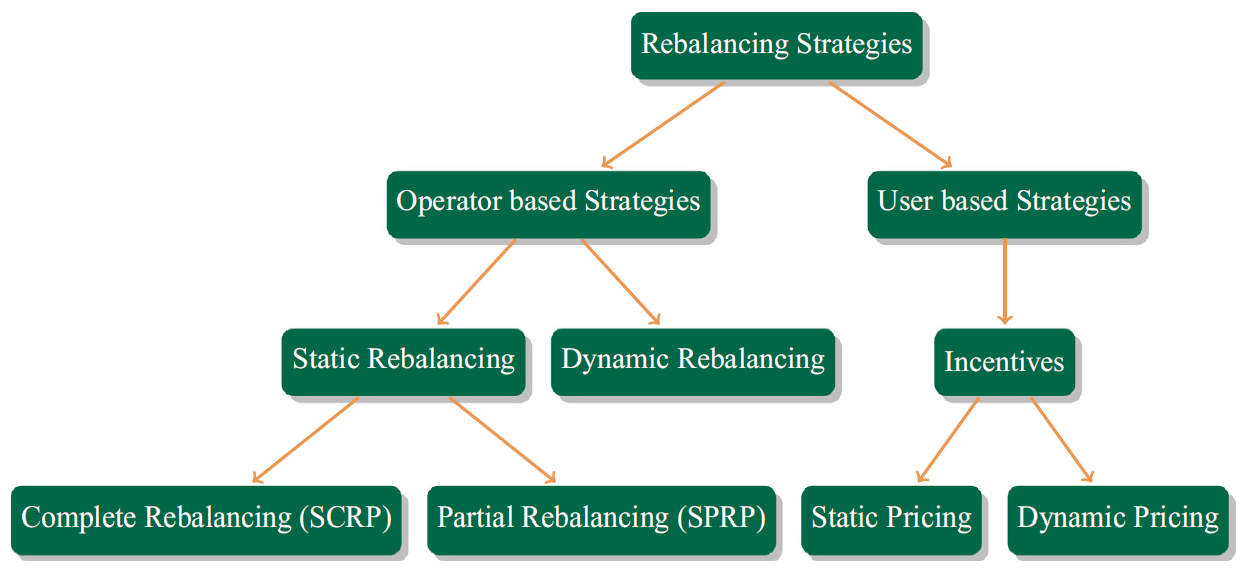
\includegraphics[width=\linewidth]{rebalancing_strategies.png}
%\caption{Overview of bike rebalancing strategies \cite{pal_zhang}.}
%\label{fig1}
%\end{figure}

\subsection{Operator-Based Strategies}
Operator-based strategies involve the use of repositioning trucks to load bikes and move them from areas with excess supply to areas with shortages. When rebalancing is done at times of low or no demand (i.e. overnight) to be able to prepare for the next day's operations, it is referred to as static rebalancing, whereas continuous rebalancing throughout the course of a day is referred to as dynamic rebalancing. Static rebalancing has the advantage of truck routing not being affected by congestion and other vehicular traffic, but it does not address supply issues throughout the course of the day. Bike share operators broadly use either or both of these approaches. Static rebalancing can be further classified into complete rebalancing, where all stations get set to meet the target inventory levels, or partial rebalancing where there are still some imbalances due to constraints such as lack of rebalancing time or not enough rebalancing vehicles available. The former is referred to as the Static Complete Rebalancing Problem (SCRP) and the latter is referred to as the Static Partial Rebalancing Problem (SPRP). User based strategies involve providing incentives to users such as reduced \& negative pricing, or extra riding time to move bikes between locations of the operator's choice.

The initial approach to SCRP and SPRP was formulated by Raviv et al., and extended by Pfrommer et al. as well as several other researchers \cite{pal_zhang}\cite{raviv}\cite{pfrommer}. Raviv presented two different approaches, both of which are mixed integer linear programs with a convex objective function. The Raviv model itself is an extension of the one-commodity pickup-and-delivery travelling salesman problem (1-PDTSP) \cite{raviv}. 1-PDTSP is an extension of the travelling salesman problem (TSP), where nodes correspond to customers that can either provide or require known amounts of a single commodity, and the objective is to visit each node exactly once using a vehicle of finite capacity, and satisfy the demand at each node while minimizing the total travel distance. Since the item is considered a commodity, an item picked up from any node can be delivered to any other node requiring that item \cite{salazar}. An exact approach exists to solve 1-PDTSP for up to 50 nodes, and several other solutions using genetic algorithms and heuristics exist to solve the problem for larger numbers of nodes; the best-known approach is able to solve instances with up to 1000 nodes \cite{salazar2}. The Raviv model extends and differs from 1-PDTSP in 5 ways \cite{raviv}:

\begin{enumerate}
    \item More than one vehicle is in use
    \item Number of items for pickup/dropoff at each node is a decision variable rather than a parameter
    \item Total travel time for the task is constrained
    \item There is a time associated with picking up and unloading each item
    \item Nodes may be visited by a vehicle more than once
\end{enumerate}

Pfrommer et al. extends the Raviv model in two main ways. The first way is by including a greeedy, promising route heuristic so that each truck chooses nodes that provide the highest utility per unit of additional travel time. Secondly, they tackle the issue of including a dynamic pricing scheme to incentivize users to modify their trips and route bikes between certain stations to rebalance the system better during operations \cite{pfrommer}. Assuming a walking speed of half the cycling speed, Pfrommer et al. create a Voronoi partition to find the effective distance from a point to the closest station, and to determine which stations can be considered neighbours. The incentive to entice users to travel to a neighbouring station rather than a desired station is sampled from a uniform distribution, and customer behaviour is assumed to be rational in going to a neighbouring station if that maximizes utility. Although these works handle SCRP and SPRP for multiple vehicles, the mathematical formulation of the problem assumes only one vehicle exists. To resolve this, nodes must be decomposed into multiple redundant nodes at the same location, each with only unit absolute imbalance. In the decomposed network, the number of visits to each node will then be at most one in order to restore balance, since each unbalanced node would have a surplus or deficit of only one item \cite{pal_zhang}. However, increasing the number of nodes like this still makes the problem difficult to solve algorithmically in reasonable time since it remains NP-hard, and therefore heuristic approaches will always be needed to find feasible solutions.

To be able to predict inventory and extend rebalancing to be dynamic, Schuijbroek et al. formulate inventory levels as a Markov Decision Process (MDP) where user behaviour is non-stationary and the rates of demand at a station can change over time, but that users pickup and dropoff bikes following a time-dependent exponential distribution. Based on this, inventory at any station can be modelled as a M/M/1 queue, and the probability of a station having a certain number of bikes at any given time can be calculated. They then use heuristics and similar methods as other researchers to solve the routing problem \cite{schuijbroek}.

\subsection{User-Based Strategies}
In addition to the model developed by Pfrommer et al. which considers dynamic pricing, Fricker and Gast developed a model where users are presented a choice between two station destinations at the time of rental, with an incentive provided to go to the station with lower capacity. Their model assumes all stations have the same capacity for docking bikes, and they show that for every 25\% increase in users deciding to go to the incentivized station, the proportion of unbalanced stations in the network decreases by a factor of 10. Like Schuijbroek et al., they predict inventory levels using a MDP \cite{fricker}.

Zulqarnain et al. view the dynamic pricing problem as a bi-level decision making process, and formulate the problem as an integer program that can be solved using genetic algorithms \cite{buffalo}. The operator's objective is to minimize the number of unbalanced stations, which leads them to modify prices provided to users. Users' objective is to minimize their travel cost. Based on the incentives provided, users will modify their travel patterns to help satisfy the operator's objective. An issue our team sees with this formulation is that it assumes users will be acting rationally, and in the interest of the bike share operator; in reality, users should not be assumed as being rational \cite{kahneman}. The model does not consider user inconvenience in modifying their start or end locations, the cost of how users value their own time, and the price elasticity of demand that would get users to consider switching their trip start and end points for a high enough incentive.

For FFBS, Zhang et al. developed a dynamic pricing model which considers negative prices (i.e. paying users) to complete desired trips. They consider walking, bus travel, and biking, and associate transferring and convenience costs between and for each of these transportation methods. They partition the search space into traffic analysis zones (TAZs), physically representing transport stations near each other as clusters, and form what they call a supernetwork out of it. The supernetwork is similar to a normal graph structure, but nodes corresponding to physical locations can be repeated to account for the transport option taken to or from the node (i.e. walking, bike, or bus). The model considers providing a negative price if users go from a TAZ with oversupply to a TAZ with undersupply, and positive prices otherwise. The positive price is fixed for all journeys it applies to, and the negative price linearly relates to the level of undersupply at the destination, up to a maximum. Negative pricing is expected to lead to two types of travel pattern changes in their model; the first is that users who might have otherwise decided to walk and not use a bike become incentivized to move a bike to an undersupplied location, and the second change is that users might change their travel paths if the benefit of the negative price outweighs the inconvenience of starting/ending further away from their originally desired travel points. By incentivizing users to move a bike to an undersupplied location, that bike then becomes available for another user's trip that can bring in positive revenue, whereas previously, the second user would not have been able to make a trip. The objective of their model is to minimize disutility (considering time, money, and comfort costs per transit mode), subject to network flow constraints on the graph \cite{neg_price}.

% \begin{figure}[htb]
% 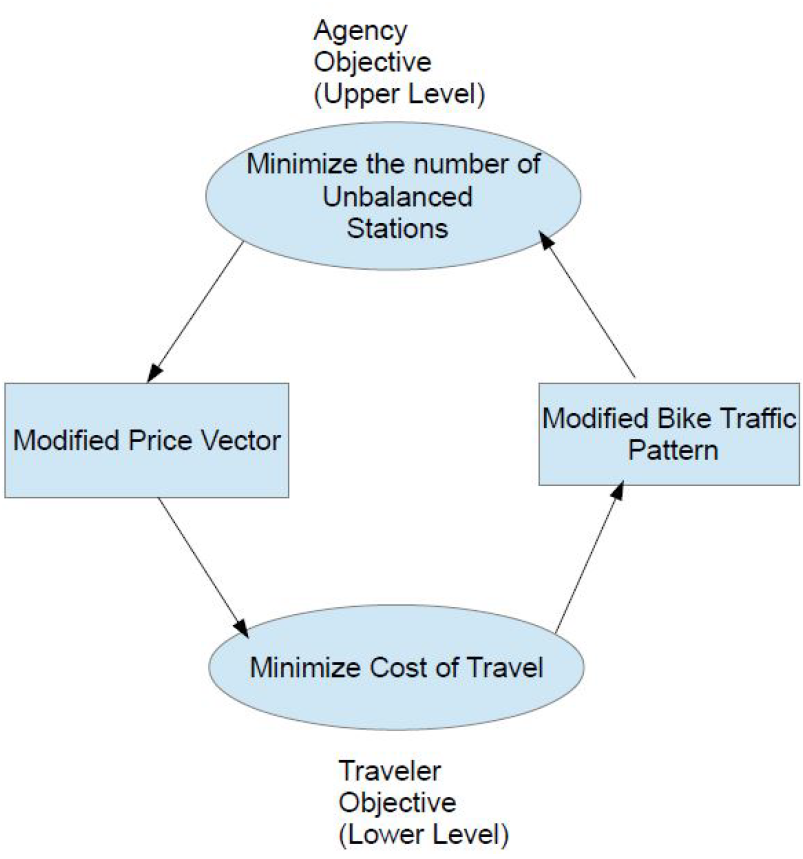
\includegraphics[width=\linewidth]{bilevel.png}
% \caption{Dynamic pricing decision making process \cite{buffalo}.}
% \label{fig2}
% \end{figure}

\section{Problem Formulation \& Modeling}
As previously discussed, the rebalancing problem can be solved by using rebalancing trucks or through dynamic pricing and user incentives. Preliminary mathematical models for each of these approaches are detailed below and will be used as a starting point to devise potential solutions for this project. 

\subsection{Operator-Based Strategies (Rebalancing)}
This problem can be formulated as follows. Each of the bike stations can be represented as a complete directed graph network, $G = (V, E)$. Here $V = \{0, ... , n\}$ is the set of vertices representing each of the stations and vertex 0 can be used to represent the bike storage facility. $E$ is the complete set of edges or routes in the directed graph, where the cost of the route $(i,j)$ can be represented by $c_{(i,j)}$. Several different objectives can be applied to represent minimizing costs, such as minimizing the total time taken for complete rebalancing, minimizing user dissatisfaction or maximizing overall system service level. The objective in this problem is to ensure that the inventory level $s_{i}$ at each station $i \in V$  satisfies $s_{i}^{min} \leq s_{i} \leq s_{i}^{max}$, where $s_{i}^{min}$ and $s_{i}^{max}$ represent minimum and maximum allowable inventories at the station. The objective function is to minimize the cost of traversing a route: 

\begin{equation}
min \sum_{(i,j)\in A}c_{ij}x_{ij}
\end{equation}

Various additional constraints can be imposed on the problem such as the maximum amount of bikes that can be picked up at any one time, or a minimum bike inventory level in the truck at all times. A complete mathematical formulation of the problem  is described in [8]. As can be seen, this is a variant of a the travelling salesman problem (TSP) which minimizes cost of the overall system rebalancing, while meeting the imposed constraints. More specifically, this is referred to as a one commodity pick up and delivery travelling salesman problem (1-PDTSP) [11]. This is because each bike station either requires pick up or delivery and the one commodity being exchanged is the bikes themselves. Based on the TSP being a NP-hard problem, the exact solution for the problem is intractable for the large number of stations and the bike fleet for which it needs to be solved. Therefore, heuristics need to be employed that could deliver approximate solutions in a reasonable amount of time.   

\subsection{User-Based Strategies (Dynamic Pricing \& Incentives)}
The user-based strategy of using dynamic pricing to influence behaviour has a similar formulation as the above mentioned operator based strategy, as it includes a component for minimum cost traversal from one station to another. This problem can be broken down into two distinct components as shown in the works of Zulqarnain et al.: a high level problem of determining the optimal price change vector to minimize the number of imbalanced stations, while the lower level problem is a minimum cost network flow problem to determine the route choice for the users [4]. The upper level pricing problem is an optimization problem to determine the price change vector, $q_{mn}$, which is used to represent the price change for traversing from the origin $i$ to the destination station $j$ using intermediary path $(m, n)$. The model objective is represented as:  

\begin{equation}
		 min \sum_{i} y_{i} + \sum_{i} z_{i}
\end{equation}

where $y_{i}$ and $z_{i}$ are binary variables representing if a station has surplus inventory or is lacking inventory. The solution minimizes the number of unbalanced stations in the whole network. In order the ensure that the unbalanced stations are minimized, a minimum cost path problem needs to be solved as follows.

\begin{equation}
min \sum_{(i,j)\in W} \sum_{(m,n) \in A_{(i,i)}}c_{mn}^{ij}x_{mn}^{ij}
\end{equation}

Here $(m, n)$ represents the neighborhood bike stations that can be used to balance supply for the origin and destination pair $(i, j)$. The cost matrix $c_{mn}^{ij}$ includes the cost of traversal from station to station including walking to any neighborhood stations if incentivized. Similar to the operator based strategy, several constraints can be applied to the problem in terms of max / min inventory levels, incentive bounds, etc. Again, based on the constraints that are defined and the numerical constants such as a number of stations, bikes available etc, the exact solution is infeasible to compute. Heuristics are required in order to simplify the problem and get a tractable solution. An example of a heuristic used by Zulqarnain et al. divides the stations into various categories ranging from highly imbalanced to completely balanced and applies the objective function on these stations for a fixed number of iterations, to compute a solution in a reasonable time period [4]. 

\begin{thebibliography}{00}

\bibitem{khamis} A. Khamis, ``4.5 - Micromobility,'' in \emph{Smart mobility: Exploring foundational technologies and wider impacts}, New York, NY: Apress, 2021, pp. 93–94. 

\bibitem{tbs_pricing} ``Pass Options,'' \emph{Bike Share Toronto}. [Online]. Available: https://bikesharetoronto.com/pricing/. [Accessed: Oct. 16, 2022]. 

\bibitem{tbs_costs} J. Hanna, ``Bike Share Business Update Q2 YTD,'' \emph{Toronto.ca}, Jul. 26, 2022. [Online]. Available: https://www.toronto.ca/legdocs/mmis/2022/pa/bgrd/backgroundfile-229023.pdf. [Accessed: Oct. 16, 2022]. 

\bibitem{buffalo}Z. Haider, A. Nikolaev, J. Kang and C. Kwon, "Real-time Dynamic Pricing for Bicycle Sharing Programs", U.S. Department of Transportation, 2014. [Online]. Available: http://utrc2.org/sites/default/files/Final-Report-Real-time-Dynamic-Pricing-Bicycle-Sharing.pdf. [Accessed Oct. 16, 2022].

\bibitem{neg_price}J. Zhang, M. Meng, and D. Z. W. Wang, ``A dynamic pricing scheme with negative prices in dockless bike sharing systems,'' \emph{Transportation Research Part B: Methodological}, vol. 127, pp. 201–224, 2019. 

\bibitem{demaio}P. DeMaio, ``Bike-sharing: History, impacts, models of provision, and future,'' \emph{Journal of Public Transportation}, vol. 12, no. 4, pp. 41–56, 2009. 

\bibitem{pal_zhang}A. Pal and Y. Zhang, ``Free-floating bike sharing: Solving real-life large-scale static rebalancing problems,'' \emph{Transportation Research Part C: Emerging Technologies}, vol. 80, pp. 92–116, 2017. 

\bibitem{raviv}T. Raviv, M. Tzur, and I. A. Forma, ``Static repositioning in a bike-sharing system: Models and solution approaches,'' \emph{EURO Journal on Transportation and Logistics}, vol. 2, no. 3, pp. 187–229, 2013. 

\bibitem{pfrommer}J. Pfrommer, J. Warrington, G. Schildbach and M. Morari, ``Dynamic Vehicle Redistribution and Online Price Incentives in Shared Mobility Systems,'' \emph{Transactions on Intelligent Transportation Systems}, vol. 15, no. 4, pp. 1567–1578, 2014. 

\bibitem{salazar}H. Hernández-Pérez and J.-J. Salazar-González, ``The one-commodity pickup-and-delivery travelling salesman problem,'' \emph{Combinatorial Optimization — Eureka, You Shrink}, pp. 89–104, 2003.

\bibitem{salazar2}H. Hernández-Pérez, I. Rodríguez Martín, and J.-J. Salazar-González, ``Introduction to Pickup-and-Delivery Problems,'' \emph{Pickup-and-delivery site}, 30-Dec-2020. [Online]. Available: http://hhperez.webs.ull.es/PDsite/\#:\%20:text=The\%201\%2DPDTSP\%20 is\%20a,minimizing\%20the\%20total\%20travel\%20distance. [Accessed: Oct. 16, 2022]. 

\bibitem{schuijbroek}J. Schuijbroek, R. C. Hampshire, and W.-J. van Hoeve, ``Inventory rebalancing and vehicle routing in bike sharing systems,'' \emph{European Journal of Operational Research}, vol. 257, no. 3, pp. 992–1004, 2017. 

\bibitem{fricker}C. Fricker and N. Gast, ``Incentives and redistribution in homogeneous bike-sharing systems with stations of finite capacity,'' \emph{EURO Journal on Transportation and Logistics}, vol. 5, no. 3, pp. 261–291, 2016. 

\bibitem{kahneman}D. Kahneman, ``Maps of Bounded Rationality: Psychology for Behavioral Economics,'' \emph{The American Economic Review}, vol. 93, no. 5, pp. 1449–1475, 2003. 

\end{thebibliography}

\end{document}